% Auteur : Romain TESTUD
\begin{frame}{Le protocole Wormhole}
    \begin{block}{Mise en contexte}
        \begin{itemize}
            \item Solution d'échanges inter-blockchains.
            \item utilisation de bridges.
        \end{itemize}
    \end{block}
    \pause
    \begin{block}{Les étapes d'un transfert}
        \begin{itemize}
            \item Formulation de la transaction.
            \item Récupération et vérification des signatures des gardiens.
            \item Envoi de la transaction.
        \end{itemize}
    \end{block}
    \begin{figure}
        \centering
        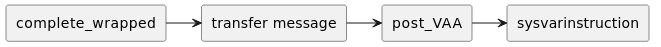
\includegraphics[scale = 0.3]{centralisation/img/fonctions.png}
        \caption{Fonctions appelées lors d'un transfert}
    \end{figure}
\end{frame}

\begin{frame}{L'attaque}
    \begin{block}{Attaque sur le bridge entre Solana et Ethereum}
        \begin{itemize}
            \item Le 2 Février 2022.
            \item 120 000 ETH de perte.
            \item Correction de bug publié mais pas encore en production.
        \end{itemize}
    \end{block}
\end{frame}

\begin{frame}{L'attaque}
    \begin{block}{Passer la signature des gardiens?}
        Utilisation de signatures d'une transaction antérieure.
    \end{block}
    \pause
    \begin{block}{Passer la vérification ?}
        \begin{itemize}
            \item Exploitation d'une erreur d'implémentation dans \textit{verify\_signature}
            \item Appel à un programme externe.
        \end{itemize}
        \begin{figure}
            \centering
            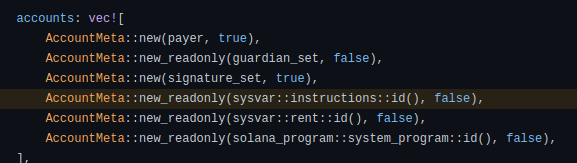
\includegraphics[scale = 0.3]{centralisation/img/sysvar_atk.png}
            \caption{Appel à la fonction de vérification}
        \end{figure}
    \end{block}
\end{frame}

\begin{frame}{L'attaque}
    \begin{itemize}
        \item Utilisation d'une nouvelle adresse.
        \item Validation des signatures par défaut.
    \end{itemize}
    \begin{figure}
        \centering
        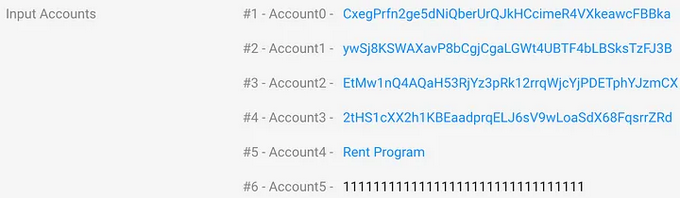
\includegraphics[scale = 0.3]{centralisation/img/sysvar_transaction.png}
        \caption{Appel à la fonction de vérification}
    \end{figure}
\end{frame}

\begin{frame}
    \begin{block}{Transaction validée et envoyée}
        \begin{itemize}
            \item 120 000 ETH transmis.
            \item Sans avoir déposé de jetons au préalable.
        \end{itemize}
    \end{block}
\end{frame}

\begin{frame}{Correctif}
    \begin{itemize}
        \item Vérification de l'appel par \textit{sysvar\_instruction}
    \end{itemize}
    \begin{figure}
        \centering
        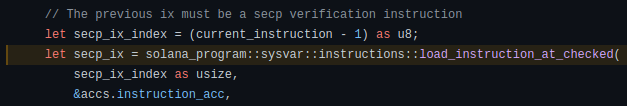
\includegraphics[scale = 0.3]{centralisation/img/worm_fixed.png}
        \caption{Appel à la fonction de vérification}
    \end{figure}
\end{frame}

%\begin{frame}
%    Etapes de transfer
%    \begin{itemize}
%        \item Vérification des signatures 
%        \item post\_vaa appelle la fonction verify signature
%        \item Verification effectuée par un programme de solana 
%        \item image des input dans le code %https://github.com/wormhole-foundation/wormhole/blob/91296e67722032debf04e95c71b3d701d4625c5b/solana/bridge/program/src/instructions.rs#L153
%    \end{itemize}
%\end{frame}

%\begin{frame}
%    Erreur d'implémentation dans verify signature
%    \begin{itemize}
%        \item Pas de vérification du programme renseigné
%        \item possibilité d'utiliser un programme externe
%    \end{itemize}
%\end{frame}
%
%\begin{frame}
%    Correction de l'erreur
%    \begin{itemize}
%        \item Commit pushed le 2 Fevrier
%        \item change load........ rajoute checked
%        \item Confirme l'utilisation du programme interne
%        \item qqun observait le git en attendant un push interessant
%    \end{itemize}
%\end{frame}
%
%\begin{frame}
%    Besoins (???) de l'attaque
%    \begin{itemize}
%        \item passer la collection des signatures
%        \item passer la vérification des signatures
%    \end{itemize}    
%\end{frame}
%
%\begin{frame}
%    Collection des signatures
%    \begin{itemize}
%        \item utilisation de signatures d'une ancienne transaction
%    \end{itemize}
%\end{frame}
%
%\begin{frame}
%    Vérification des signatures
%    \begin{itemize}
%        \item Exploitation de l'erreur d'implémentation de verify\_signature
%    \end{itemize}
%\end{frame}
%
%\begin{frame}
%    
%\end{frame}
%
%\begin{frame}{Wormhole}
%    Attaque sur le bridge entre Solana et Ethereum :
%    \begin{itemize}
%        \item Quelques heures après un correctif non déployé.
%        \item Exploitation d'un défaut d'implémentation.
%        \item La transaction de l'attaquant est signée par les gardiens.
%    \end{itemize}
%\end{frame}
%\begin{frame}{Wormhole}
%    \begin{block}{Fonctionnement du dépôt de jeton}
%        \begin{itemize}
%            \item Appel de plusieurs fonctions de vérification lors du dépôt.
%            \begin{itemize}
%                \item $complete\_wrapped$ $\Rightarrow$ 
%                 $transfer\_message$
%                 $\Rightarrow$  $post\_vaa$
%                 $\Rightarrow$  $verify\_signature$
%            \end{itemize}
%            %\item Fonction complete\_wrapped appellée lors du mint de Wormhole ETH sur Solana
%            %\item transfer\_message en paramètre : spécifie le token et combien doit être mint, signé par les gardiens
%            %\item Contrat sur Solana, créé en utilisant la fonction post\_vaa qui vérifie la signature des gardiens
%            %\item Appel a verify\_signature qui utilise un programme de Solana pour verifier les signatures
%        \end{itemize}
%        Erreur d'implémentation dans $verify\_signature$.
%    \end{block}
%\end{frame}
%
%\begin{frame}{Wormhole}
%    \begin{block}{$verify\_signature$ appelle un programme de vérification}
%        \begin{itemize}
%            \item $Sysvar: Instructions$ : Alias du programme.
%            \item Vérification des signatures des gardiens.
%            \item Il est possible d'utiliser d'une adresse différente.
%        \end{itemize}  
%    \end{block}
%    %\begin{figure}
%    %    \centering
%    %    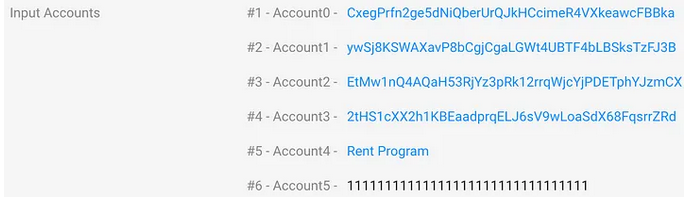
\includegraphics[scale = 0.3]{img/wormhole_img1.png}
%    %\end{figure}
%\end{frame}
%
%\begin{frame}{Wormhole}
%    \begin{itemize}
%        \item Adresse tierce entrée par l'attaquant.
%        \item Validation de la transaction sans signature.
%    \end{itemize}
%    %\begin{figure}
%        %\centering
%        %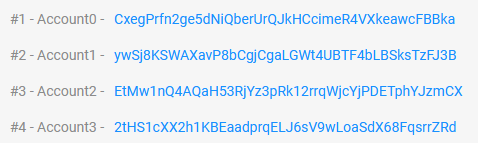
\includegraphics[scale = 0.7]{img/wormhole_img2.png}
%    %\end{figure}
%\end{frame}